The development of neural quantum states (NQS) has been deeply influenced by challenges and innovations in condensed matter physics, where strongly correlated quantum many-body systems demand accurate and scalable computational approaches. Many of the foundational ideas behind NQS, including pioneering work using restricted Boltzmann machines~\cite{carleo_solving_2017}, emerged from efforts to model lattice spin systems. These were subsequently extended to continuous-space systems such as the homogeneous electron gas~\cite{pescia_message-passing_2024} and ultracold Fermi gases~\cite{kim_neural-network_2024}. Such advances offer a natural conceptual bridge to nuclear systems, which pose many of the same computational challenges. As a general-purpose variational ansatz, NQS provides greater flexibility than traditional techniques and holds promise for systems governed by complex interactions and symmetry constraints. We now review two condensed matter NQS applications which are closely tied to nuclear approaches. These approaches employ a continuous formulation and tackle either low dimensionality or extended, strongly-correlated systems.

\subsection{Polarized fermions}
\label{sub:polarized_fermions} 


One-dimensional fermionic systems offer a particularly useful and conceptually rich setting for studying quantum many-body physics, combining analytical insight with computational accessibility.
Due to their reduced dimensionality, such systems admit simplified theoretical descriptions and, in some cases, exact or highly controlled solutions~\cite{busch_two_1998, bethe_zur_1931}, while still exhibiting nontrivial correlation effects that challenge mean-field approaches.
From a computational standpoint, one-dimensional models provide a natural proving ground for new variational methods, as they allow detailed benchmarking against established many-body techniques at modest numerical cost.
In addition, one-dimensional fermions display distinctive phenomena, such as Fermi--Bose dualities and enhanced interaction effects, that have no direct analogue in higher dimensions and are of intrinsic theoretical interest~\cite{girardeau_relationship_1960,valiente_bose-fermi_2020,girardeau_effective_2004}.
These features make one-dimensional fermionic systems an attractive platform for exploratory studies of neural-network quantum states, serving as a stepping stone toward more realistic three-dimensional and spinful systems of relevance to nuclear and condensed-matter physics~\cite{keeble_machine_2020,adams_variational_2021,gnech_nuclei_2022,lovato_hidden-nucleons_2022}.


%One-dimensional fermionic systems provide an excellent yet challenging testing ground for quantum many-body theory~\cite{1dreview}. 
%The reduced spatial dimensionality enables the existence of exact solutions in a variety of settings, including few-body trapped systems~\cite{busch_two_1998} and integrable models solvable by the Bethe ansatz~\cite{bethe_ansatz}. 
%At the same time, one-dimensional systems exhibit distinct many-body phenomena, such as fermion--boson dualities and enhanced correlation effects, that are absent or less pronounced in higher dimensions. 
%From a computational perspective, lower-dimensional settings also offer a controlled environment for developing and benchmarking new variational approaches before extending them to fully three-dimensional systems.

This strategy has been adopted in several early applications of neural-network quantum states to continuous-space fermionic systems~\cite{keeble_machine_2023,bedaque_machine_2024}. 
In particular, Ref.~\cite{keeble_machine_2023} investigated fully polarized, or equivalently spinless, fermions confined to one dimension. 
In this setting, the absence of internal spin degrees of freedom allows the fermionic antisymmetry to be enforced entirely through the spatial structure of the wave function, making it a natural test case for NQS architectures without explicit spin inputs. 
To ensure nontrivial interactions in the polarized system, finite-range pairwise forces must be employed, since zero-range interactions do not contribute to the energy of identical fermions in one dimension~\cite{keeble_machine_2023}.

The system considered in Ref.~\cite{keeble_machine_2023} consists of $A$ fermions in a harmonic trap interacting through a finite-range Gaussian potential, described by the Hamiltonian
\begin{align}
\hat H = - \frac{1}{2} \sum_{i=1}^A \nabla_i^2 
+ \frac{1}{2} \sum_{i=1}^A x_i^2
+ \frac{V_0}{\sqrt{2\pi}\sigma_0}
\sum_{i<j} \exp\!\left[-\frac{(x_i-x_j)^2}{2\sigma_0^2}\right].
\end{align}
Here, $V_0$ and $\sigma_0$ denote the interaction strength and range, respectively. 
The Hamiltonian is expressed in harmonic-oscillator units corresponding to a trap frequency $\omega$, such that lengths are measured in units of $a_{\mathrm{ho}} = \sqrt{\hbar/m\omega}$ and energies in units of $\hbar\omega$.

The NQS employed for this system was inspired by the FermiNet architecture~\cite{pfau_ab_2020}. 
In one dimension, the many-body wave function depends only on the particle coordinates $\Psi(x_1,\ldots,x_A)$. 
The neural ansatz takes as input the set of particle positions and augments them with a permutation-equivariant feature, the mean position
$\mu = \frac{1}{A}\sum_{i=1}^A x_i$. 
These features are propagated through two equivariant hidden layers with element-wise $\tanh$ nonlinearities, followed by a linear layer that constructs a symmetric generalized Slater matrix. 
The determinant of this matrix yields the full antisymmetric many-body wave function~\cite{keeble_neural_2022,keeble_machine_2023}. 
For particle numbers in the range $A=2$--$6$, this architecture contains approximately $8{,}500$--$9{,}000$ variational parameters, with only mild scaling as $A$ increases.


\begin{figure}[!t]
\centering
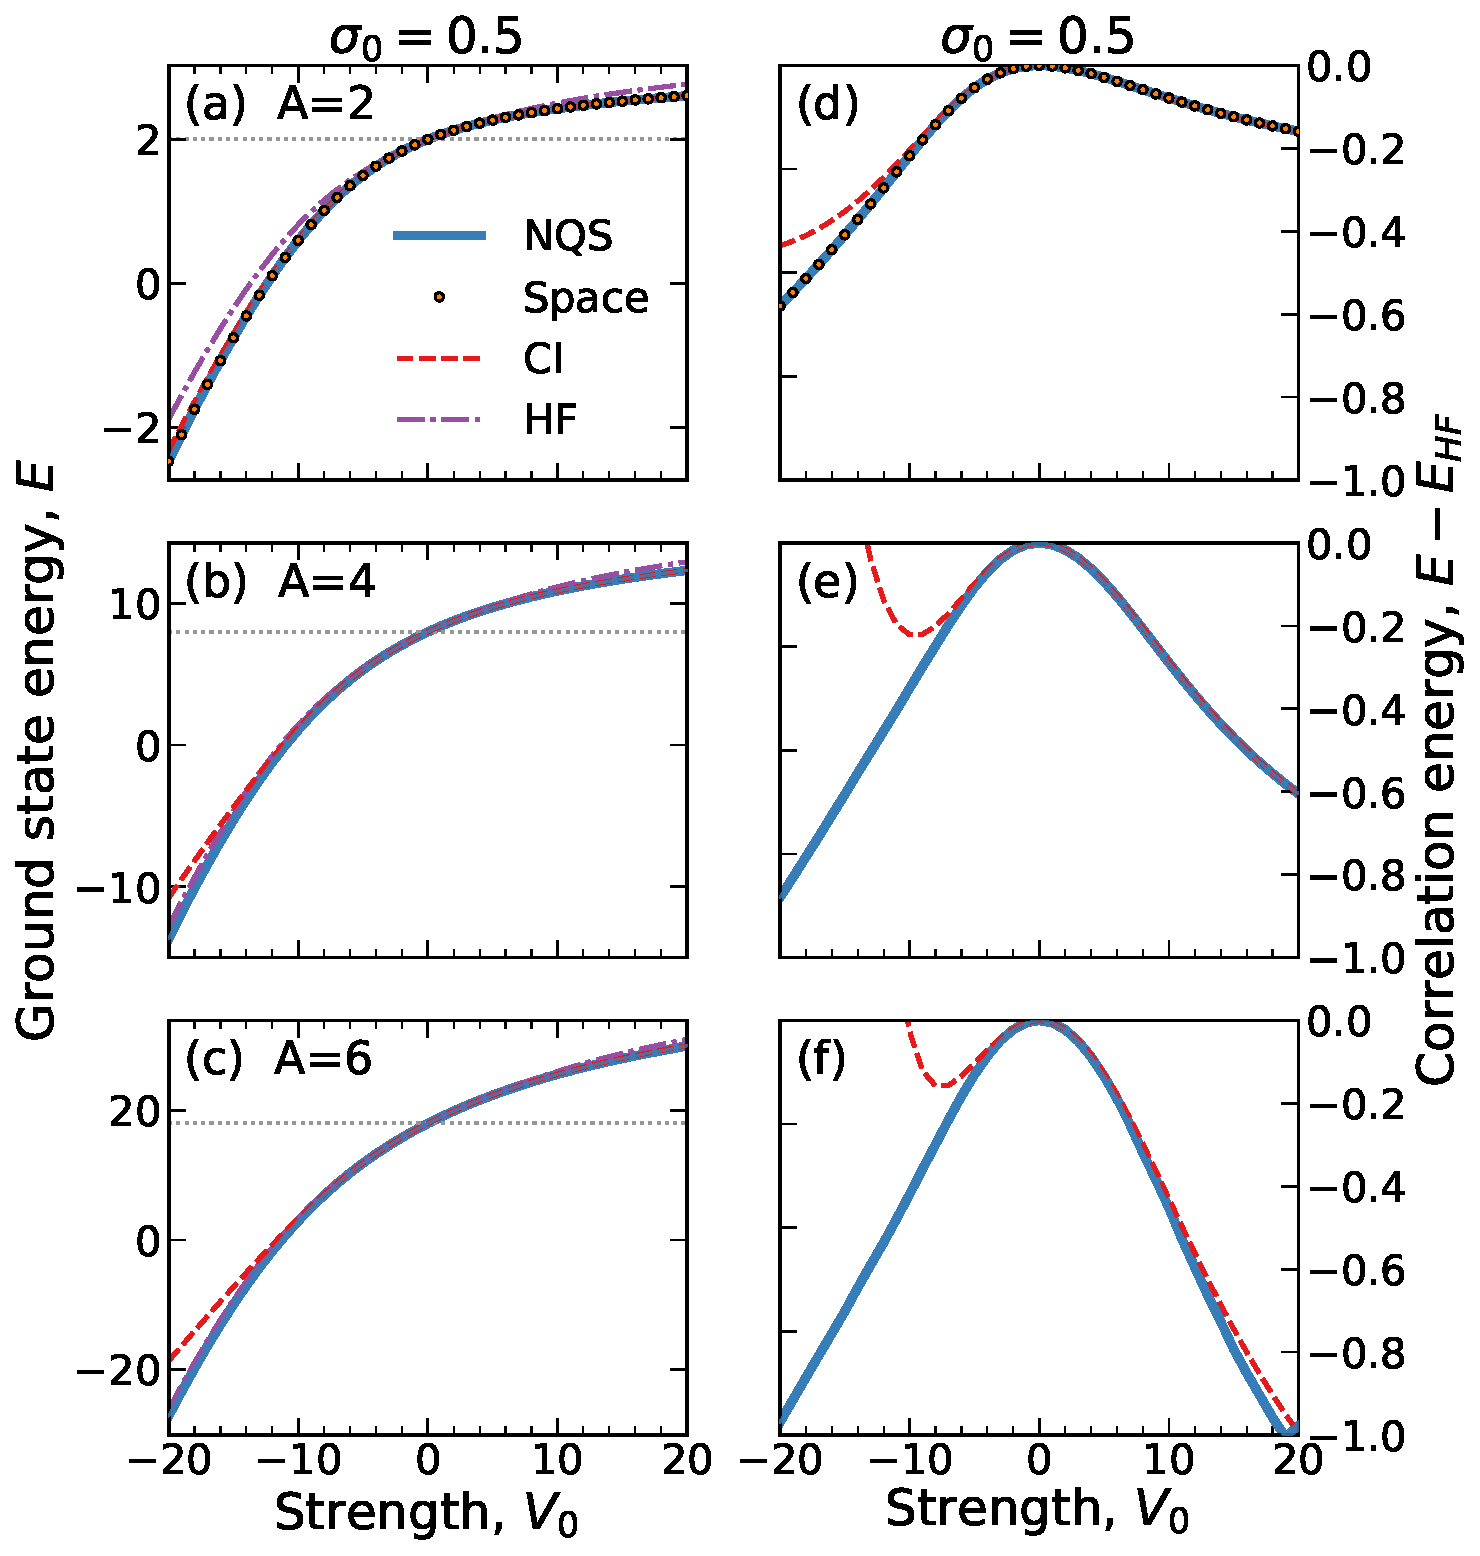
\includegraphics[width=0.5\columnwidth]{figures/condensed_matter/1D_energy_panel_review.pdf}
\caption{Ground-state energies for few-body systems as a function of the interaction
strength \(V_0\) at fixed range \(\sigma_0 = 0.5\).
Panels (a)–(c) show the total energy \(E\) for systems with
\(A = 2, 4,\) and \(6\), while panels (d)–(f) show the corresponding
correlation energies \(E - E_{\mathrm{HF}}\).
Neural-network quantum state (NQS) results are shown as solid blue lines.
The real-space solution for \(A = 2\) is indicated by filled circles.
Configuration-interaction (CI) results are shown as red dashed lines, and the
Hartree--Fock (HF) approximation as purple dash-dotted lines, following
Ref.~\cite{keeble_machine_2023}.}
\label{fig:1D_energy}
\end{figure}

In Fig.~\ref{fig:1D_energy}, NQS results are compared with configuration interaction (CI), Hartree–Fock (HF), and real-space solutions (Space), where available, for a fixed width $\sigma_0 = 0.5$. For all particle numbers $A = 2, 4,$ and $6$, the NQS yields energies below the HF results, with the discrepancy increasing as the interaction becomes either strongly attractive or strongly repulsive. This architecture only incorporates a single generalised Slater determinant, so the difference between the HF and NQS results can directly be linked to backflow correlations included by construction through the equivariant features. 

While the NQS performs consistently across all interaction regimes and reproduces the exact results for $A = 2$, the fixed-dimension CI calculations exhibit noticeable basis-truncation effects as the interaction strength increases, particularly in the attractive regime. This behavior can be traced to the emergence of short-range structure in the wave function under strong attraction. Resolving accurately these structure requires progressively larger single-particle bases. 

The density distributions of one-dimensional systems directly pinpoint the effect of complex many-body correlations. We show in Fig.~\ref{fig:1D_densities} the density distributions across a wide range of strengths, from very attractive (left panels) to very repulsive (right panels). The repulsive regime can be easily understood in terms of Wigner crystallization~\cite{keeble_machine_2023}. In contrast, the density distribution in the strongly attractive regime
%not shown here in the interest of brevity, 
displays a distinct bell shape that is reminiscent of bosonic systems. An associated pairing-like effect in the occupation numbers of the system further points towards the emergence of bosonic features in the many-body wavefunction~\cite{keeble_machine_2023}. CI approaches have a difficulty capturing such results. These features, however, can be understood in terms of a duality between strongly attractive fermions and weakly interacting bosons in 1D systems~\cite{girardeau_relationship_1960,valiente_bose-fermi_2020,girardeau_effective_2004}. 
Overall, these results demonstrate that relatively compact, permutation-equivariant NQS architectures can capture strong-correlation effects in continuous-space fermionic systems. 
The one-dimensional exactly solvable case thus provides a clean benchmark and a foundation for extensions to higher-dimensional and spinful systems.

\begin{figure}[!t]
\centering
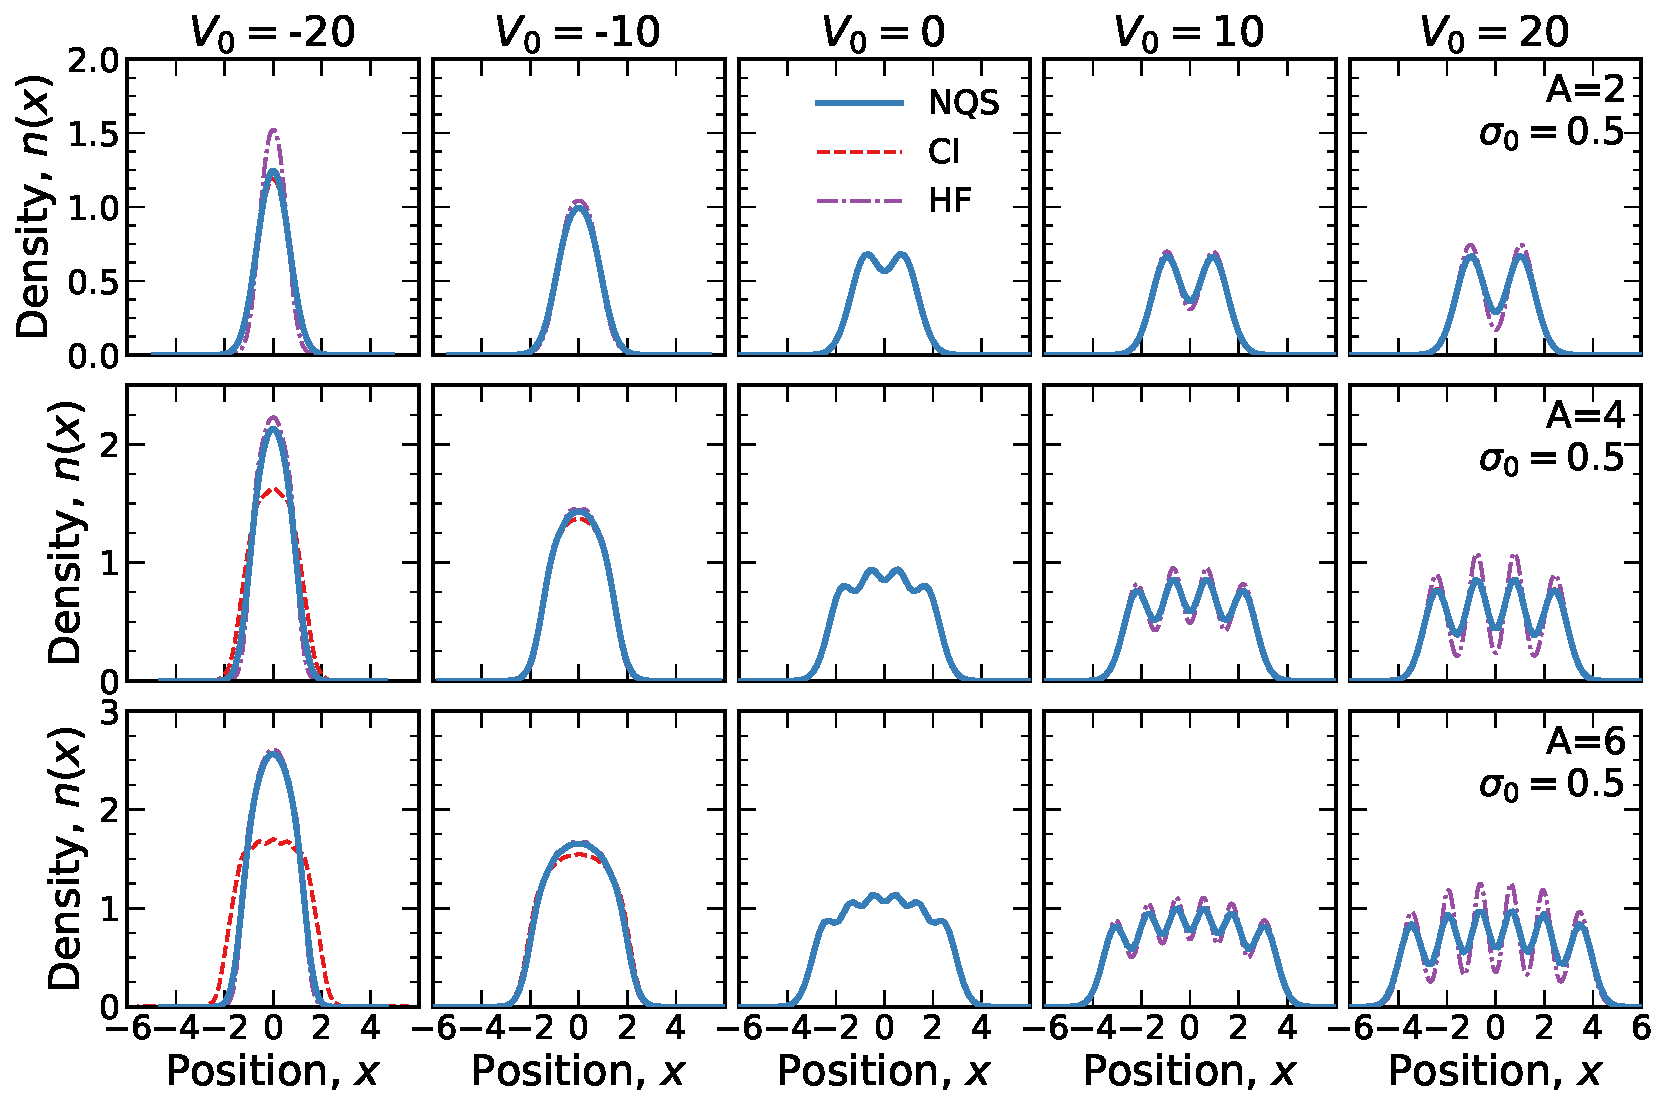
\includegraphics[width=0.8\columnwidth]{figures/condensed_matter/1D_density_panel_review.pdf}
\caption{Density profiles \(n(x)\) for one-dimensional spinless trapped fermions as a function of position \(x\) for different values
of \(V_0\) at fixed range \(\sigma_0 = 0.5\). From left to right, \(V_0\) varies
from \(-20\) to \(20\) in increments of 10. From top to bottom, results are
shown for \(A = 3, 4, 5,\) and \(6\) particles. Figure sourced from Ref.~\cite{keeble_machine_2023}.}
\label{fig:1D_densities}
\end{figure}


\subsection{The homogeneous electron gas}
\label{sub:heg}

The three-dimensional homogeneous electron gas (HEG) has long served as a prototypical model for studying strongly correlated fermions with long-range Coulomb interactions. Despite its apparent simplicity, with electrons interacting via the Coulomb potential in a uniform, neutralizing background, the HEG exhibits rich many-body behavior. At low densities, where Coulomb repulsion dominates over kinetic energy, the system is expected to undergo Wigner crystallization into a body-centered cubic (BCC) lattice. Due to translational invariance, this crystal may appear as a ``floating'' phase, characterized by crystalline order in correlations rather than in the density itself.

The HEG has been investigated with a variety of NQS architectures in recent years, including
LiNet~\cite{li_ab_2022}, FermiNet~\cite{cassella_discovering_2023}, and WAPNet~\cite{wilson_neural_2023}, as well as with conventional many-body methods such as diffusion Monte Carlo~\cite{lopez_rios_inhomogeneous_2006,azadi_low-density_2022} and coupled cluster approaches~\cite{liao_towards_2021}.
Rather than surveying these applications exhaustively, we focus here on the approach of Ref.~\cite{pescia_message-passing_2024}, for which the HEG served as the primary development and validation platform for the permutation-equivariant message-passing neural network (MPNN) architecture that appears throughout this review.
The insights gained in this setting subsequently informed applications to other continuous-space fermionic systems, including ultracold Fermi gases~\cite{kim_neural-network_2024}, nuclear matter~\cite{fore_investigating_2024}, and finite nuclei~\cite{gnech_distilling_2024,donna_hypernuclei_2025}.

To resolve the emergence of the floating Wigner crystal, NQS must scale to large particle numbers while accurately capturing subtle many-body correlations.
This requirement directly motivated the development of a permutation-equivariant MPNN architecture augmented with an attention mechanism~\cite{pescia_message-passing_2024}, which encodes how the state of a single electron is influenced by the instantaneous positions and spins of all other electrons.
This approach enabled simulations of the HEG with up to 128 electrons, pushing far beyond the system sizes accessible in previous NQS studies~\cite{li_ab_2022}, and made it possible to detect Wigner-like order in the structure factor at low densities (see Fig.~\ref{fig:heg}).

In this HEG application, the construction of the MPNN begins by representing each electron as a node in a fully connected graph, with edges encoding the pairwise relationships between electrons. The goal of the MPNN is to produce spatial displacements $\delta \mathbf{r}_i(\mathbf{X})$ for each particle $i = 1, \ldots, N$, thereby incorporating backflow correlations into the single-particle orbitals of a neural Slater determinant. During each message-passing iteration, both the original one- and two-body features from the simulation and a set of auxiliary hidden one- and two-body vectors are propagated and updated, enabling the network to progressively refine its representation of correlations. Specifically, the visible two-body features for the HEG are taken to be
\begin{equation}
    \mathbf{v}_{ij} = \big[ \mathbf{r}_{ij}, \ \| \mathbf{r}_{ij} \|, \ s_i^z \cdot s_j^z \big],
\end{equation}
where the pair displacements $\mathbf{r}_{ij} = \mathbf{r}_i - \mathbf{r}_j$ and distances $\|\mathbf{r}_{ij}\|$ are mapped to their $L$-periodic versions:
\begin{align}
    \mathbf{r}_{ij} \ \mapsto \ 
    \left[ 
    \sin \left( \frac{2 \pi}{L} \mathbf{r}_{ij} \right),
    \cos \left( \frac{2 \pi}{L} \mathbf{r}_{ij} \right) \right], \quad
    \|\mathbf{r}_{ij}\| \ \mapsto \
    \Bigg\| \sin\left(\frac{\pi}{L} \mathbf{r}_{ij} \right) \Bigg\|.
\end{align}
The initial one-body features, on the other hand, are taken as a trainable embedding vector that is independent of the particle index,
\begin{equation}
    \mathbf{v}_i = \mathbf{e}.
\end{equation}
Note that this choice of initial one-body features excludes dependence on absolute positions $\mathbf{r}_i$ to ensure translational invariance.


\begin{figure}[!t]
\centering
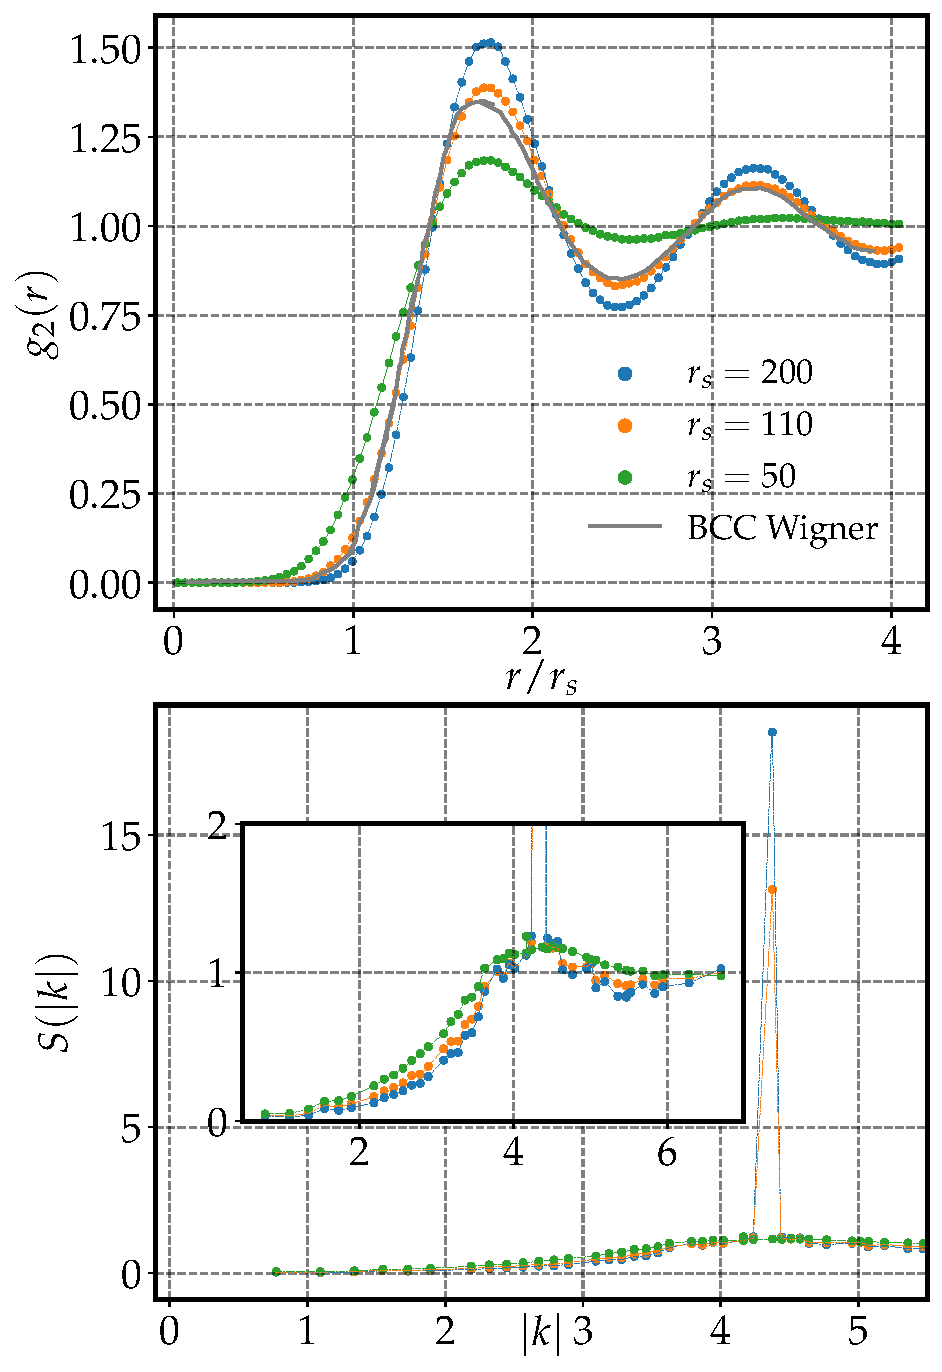
\includegraphics[width=0.5\columnwidth]{figures/condensed_matter/g2_Sk_128_nolog_2panel.pdf}
\caption{Spin-averaged radial distribution function (top panel) and the corresponding
structure factor (bottom panel) for the homogeneous electron gas with
\(N = 128\) electrons, evaluated at \(r_s = 50, 110,\) and \(200\).
A permutation-equivariant message-passing neural network with an attention
mechanism~\cite{pescia_message-passing_2024} was used to construct backflow
correlations within a Slater--Jastrow NQS. Plane-wave orbitals were used at
\(r_s = 50\), while Gaussian orbitals centered on body-centered cubic (BCC)
lattice sites were employed at \(r_s = 110\) and \(200\). }
\label{fig:heg}
\end{figure}

Beyond the initial one- and two-body features and their processing into visible features, the main difference between this MPNN and the one in Section~\ref{subsub:backflow_correlations} is the use of an attention mechanism~\cite{vaswani_attention_2017} in the message construction. Originally developed for natural language processing, attention mechanisms learn to assign weights to different inputs, enabling the model to focus on the most relevant information when updating each particle's features (see Section~\ref{sec:deep_learning} for more details).
Unlike Eq.~\eqref{eq:mpnn-message}, where a feedforward neural network is applied directly to the pairwise features to produce the message, Ref.~\cite{pescia_message-passing_2024} first computes an attention score
\begin{equation}
    \boldsymbol{\omega}_{ij}^{(t)} = \mathrm{GELU}
    \left(\sum_{k=1}^N \mathbf{Q}_{ik}^{(t)} \mathbf{K}_{kj}^{(t)} \right),
\end{equation}
which modulates the signal element-wise based on similarities between the query tensor $\mathbf{Q}_{ij}^{(t)} = W_Q \mathbf{g}_{ij}^{(t)}$ and the key tensor $\mathbf{K}_{ij}^{(t)} = W_K \mathbf{g}_{ij}^{(t)}$.
Note that the weight matrices used to produce the query and key are the same for each pair to ensure permutation equivariance.
The message is then constructed as
\begin{equation}
    \mathbf{m}_{ij}^{(t)} = \boldsymbol{\omega}_{ij}^{(t)} \odot f_V^{(t)}(\mathbf{h}_{ij}^{(t-1)}),
\end{equation}
where $f_V^{(t)}$ serves as the value network, providing the information to be passed through a nonlinear transformation, and $\odot$ denotes element-wise multiplication rather than the usual dot product. This construction provides flexibility in defining the message content while simultaneously weighting its relevance.

The MPNN approach achieves ground-state energies for the HEG that are on par with or better than those obtained with state-of-the-art NQS, such as FermiNet~\cite{cassella_discovering_2023} and WAPNet~\cite{wilson_neural_2023}, as well as fixed-node and backflow diffusion Monte Carlo methods~\cite{lopez_rios_inhomogeneous_2006, azadi_low-density_2022}. For small systems, it reaches chemical accuracy relative to exact methods, while for larger systems it outperforms comparable variational and diffusion Monte Carlo approaches, particularly at high densities. The method systematically improves with additional message-passing iterations and maintains accuracy across different densities and polarizations. Most notably, the MPNN uses orders of magnitude fewer parameters ($\sim 19{,}000$) than other NQS, and can simulate continuous-space systems with up to 128 electrons, more than double the size previously accessible.

The method also reproduces the expected liquid-to-Wigner-crystal phase transition around $r_s = 100$, in agreement with previous studies~\cite{azadi_correlation_2023,drummond_diffusion_2004, ceperley_ground_1980}. Gaussian orbitals were found to more easily capture the crystalline phase for large $r_s$ compared to plane-wave orbitals, as shown in Fig.~\ref{fig:heg}. The prominent peak in the structure factor that appears between $r_s = 50$ and $r_s = 110$ indicates the emergence of a crystalline state from a fluid state. These results demonstrate that MPNN-based NQS can efficiently and accurately model both delocalized and localized phases in extended systems, providing a framework applicable to other systems where backflow correlations play a central role.

\subsection{Ultra-cold Fermi gases}
\label{sub:ufg}

The unitary Fermi gas (UFG) is a paradigmatic strongly correlated quantum system of two-component fermions interacting via a short-range potential tuned to infinite scattering length and negligible effective range. In this regime, the system exhibits universal behavior, with properties determined solely by the particle density rather than the microscopic details of the interaction. The UFG lies at the crossover between the BCS superfluid and the Bose--Einstein condensate (BEC) limits, and displays strong pairing correlations and superfluidity in the absence of a small expansion parameter. These features make the UFG both a challenging nonperturbative many-body problem and an ideal benchmark for testing wave-function ans\"atze and many-body methods. Moreover, low-density neutron matter in the inner crust of neutron stars shares similar universal characteristics, making the UFG a useful proxy for studying pairing and superfluidity in astrophysical systems.

In this review, we focus on the work of Ref.~\cite{kim_neural-network_2024}, which introduces a Pfaffian--Jastrow NQS augmented by neural backflow transformations generated through a permutation-equivariant message-passing architecture~\cite{pescia_message-passing_2024}. This construction combines a fully trainable Pfaffian pairing structure with many-body backflow effects, enabling the wave function to capture fermionic antisymmetry and strong pairing correlations within a unified framework, without imposing a predefined decomposition into singlet and triplet pairing channels, fixed functional forms for the pairing orbitals, or a prescribed spin ordering. As a result, the ansatz can be naturally extended to nuclear systems with explicit spin- and isospin-exchange interactions and nontrivial coupling to the spatial degrees of freedom. In parallel with  Ref.~\cite{kim_neural-network_2024}, an NQS approach to the unitary Fermi gas based on the FermiNet architecture was developed around the same time~\cite{lou_neural_2024}. However, its formulation targets systems with fixed internal spin degrees of freedom and can not directly address the explicit spin--isospin exchange structure of nuclear interactions.

\iffalse
\begin{figure}[!t]
\centering
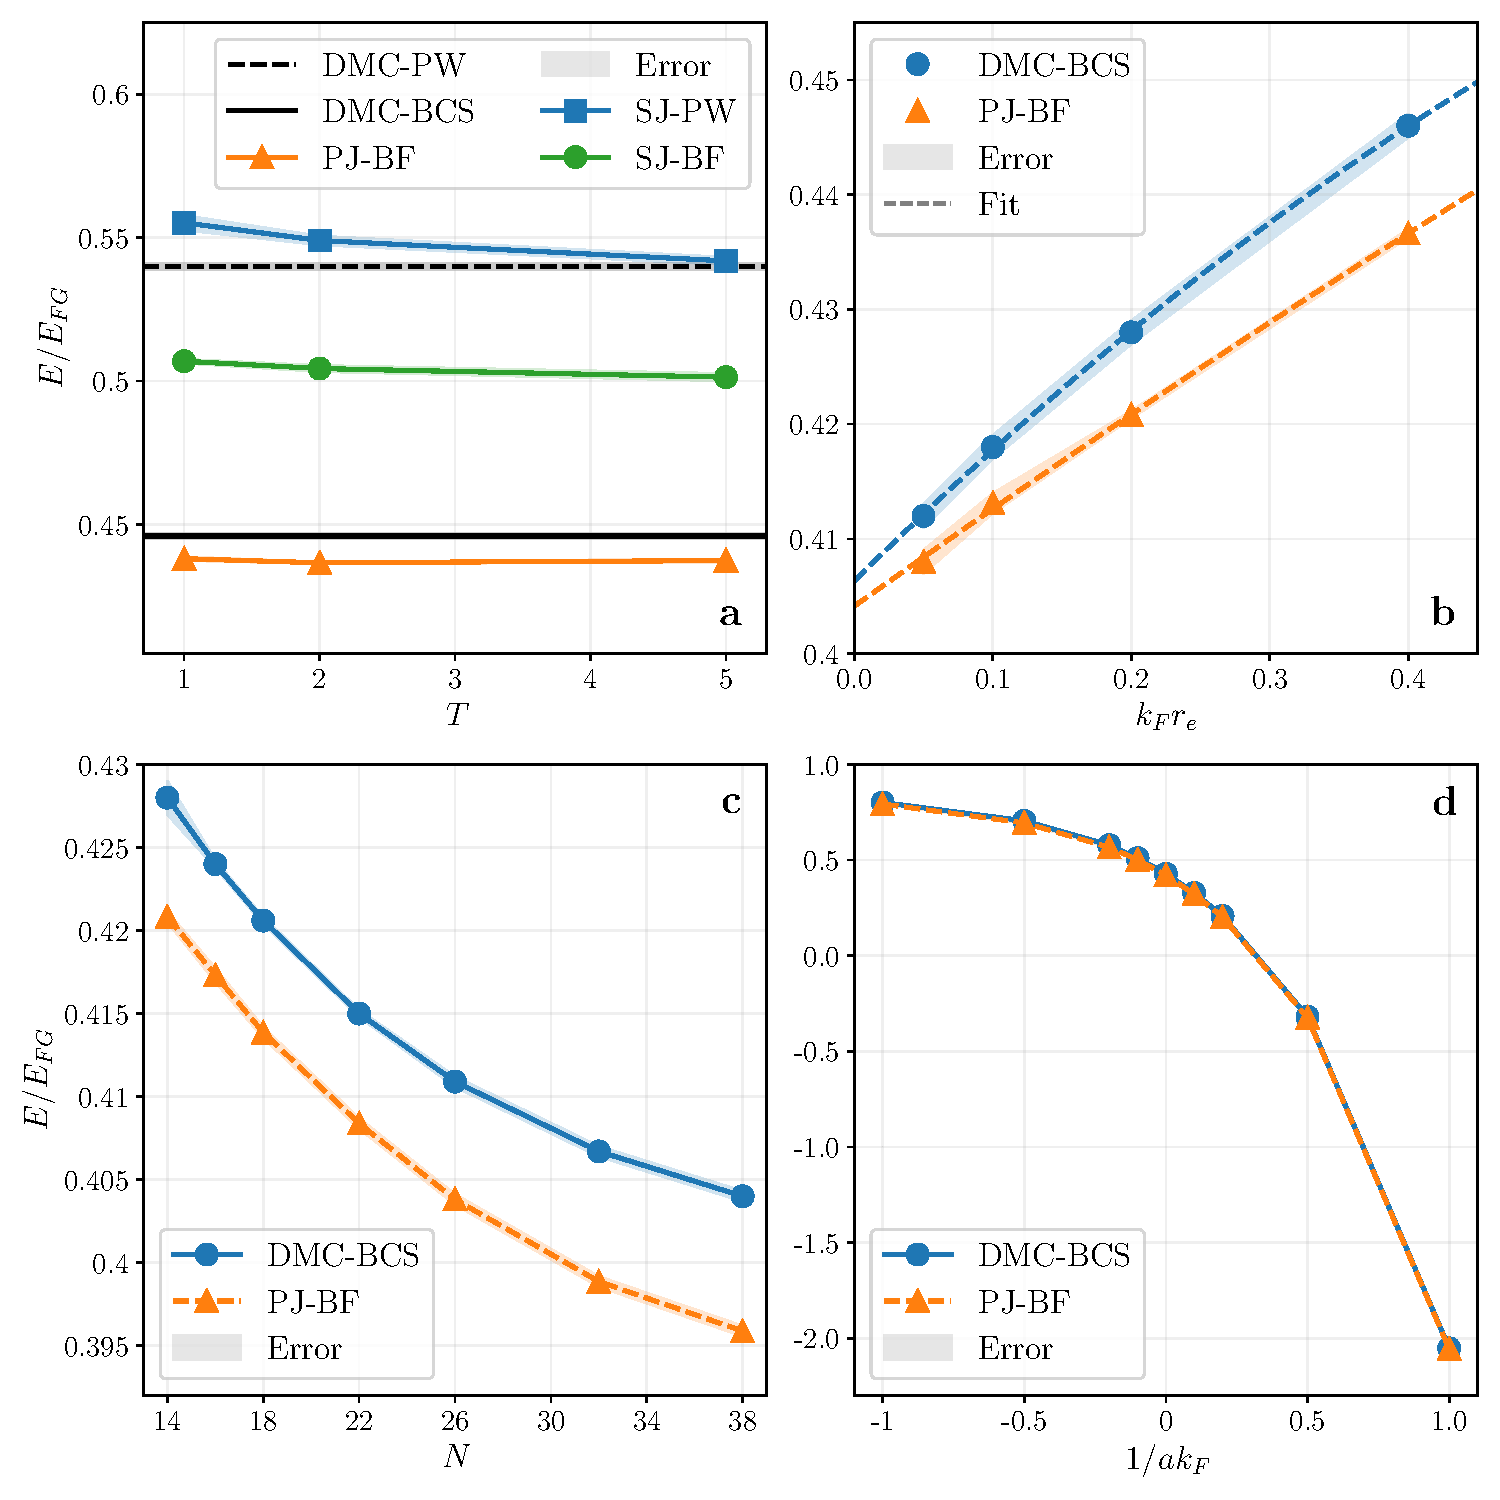
\includegraphics[width=0.75\columnwidth]{figures/condensed_matter/energies.pdf}
\caption{
Ground-state energy per particle for the unitary Fermi gas, normalized by the
noninteracting Fermi gas energy in the thermodynamic limit.
For the NQS results, converged energies are
obtained by averaging over the final 100 optimization iterations, with shaded
bands indicating the corresponding standard deviations. For the diffusion
Monte Carlo (DMC) data, uncertainty bands represent the standard errors from
block-averaged energies. The Pfaffian--Jastrow ansatz with backflow (PJ--BF) is
shown as orange triangles in all panels.
All numerical values can be found in Ref.~\cite{kim_neural-network_2024}.
\textbf{a} Initial comparison of three NQS architectures and two DMC
benchmarks as a function of the message-passing neural network depth \(T\).
The Slater--Jastrow ansatz with plane-wave orbitals (SJ--PW) is indicated by
blue squares, while the Slater--Jastrow ansatz with backflow (SJ--BF) is shown
as green circles. Interaction parameters are fixed to \(v_0 = 1\) and
\(\mu = 5\), corresponding to an effective range \(k_F r_e = 0.4\). DMC
reference energies with pairing (DMC--BCS) and without pairing (DMC--PW) are
displayed as solid and dashed curves, respectively.
\textbf{b} Energies at unitarity as a function of the effective range
\(k_F r_e\). The DMC--BCS benchmark values (blue circles) and PJ--BF results
(orange triangles) are extrapolated to zero effective range using quadratic
fits, shown as dashed lines. 
\textbf{c} Energies at unitarity versus particle number \(N\) (even values
only), with the effective range fixed to \(k_F r_e = 0.2\).
\textbf{d} Energies across the BCS--BEC crossover as a function of the
inverse scattering length \(1/a k_F\) at fixed effective range
\(k_F r_e = 0.2\).}
\label{fig:ufg-energies}
\end{figure}
\fi

\begin{figure}[!t]
\centering
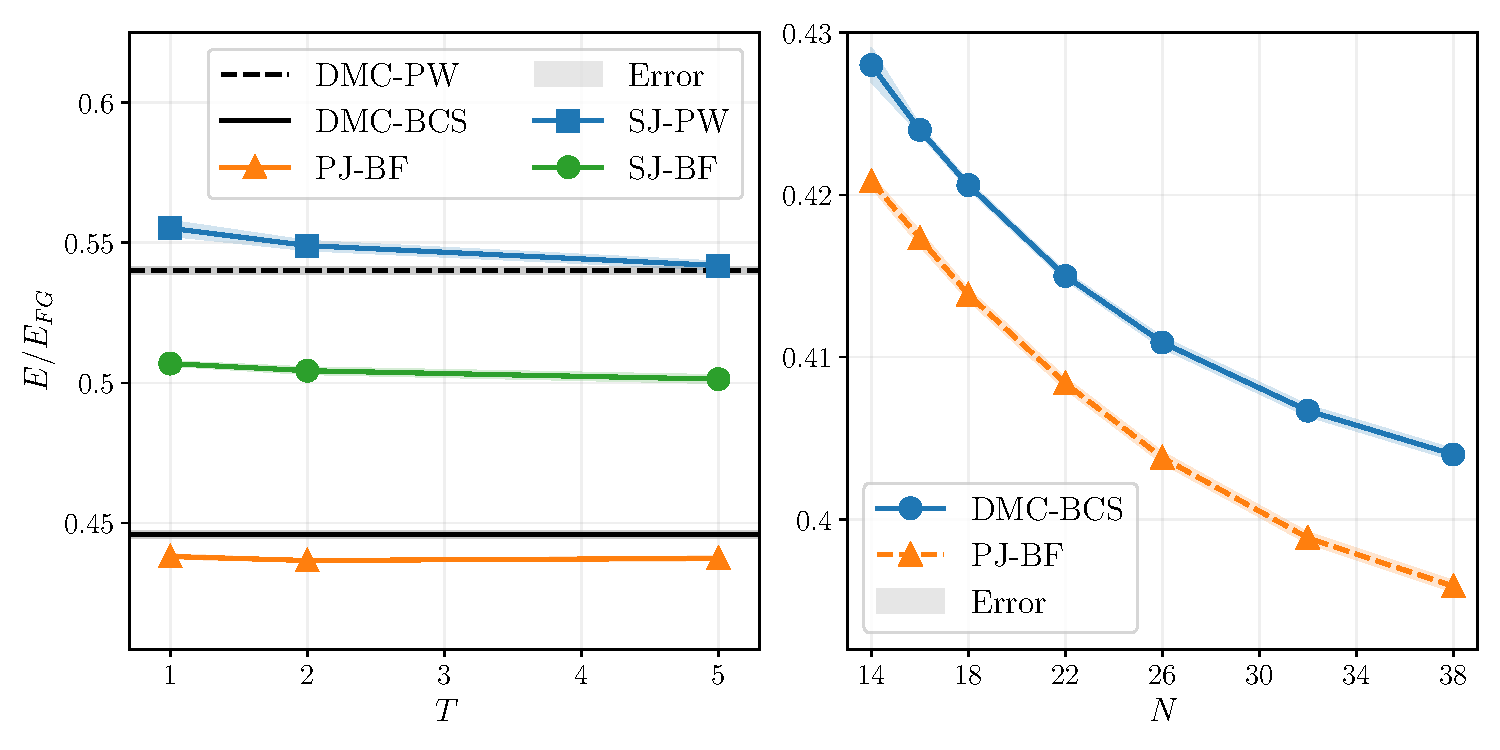
\includegraphics[width=0.75\columnwidth]{figures/condensed_matter/energies_T_N.pdf}
\caption{
Ground-state energy per particle of the UFG, normalized by the noninteracting Fermi gas energy in the thermodynamic limit, $E_{FG}$, as a function of message-passing depth \(T\) (left panel) and particle number \(N\) (right panel).
Details of the models, interaction parameters, and uncertainty estimates are discussed in the main text.
}
\label{fig:ufg-energies-T-N}
\end{figure}

\begin{figure}[!t]
\centering
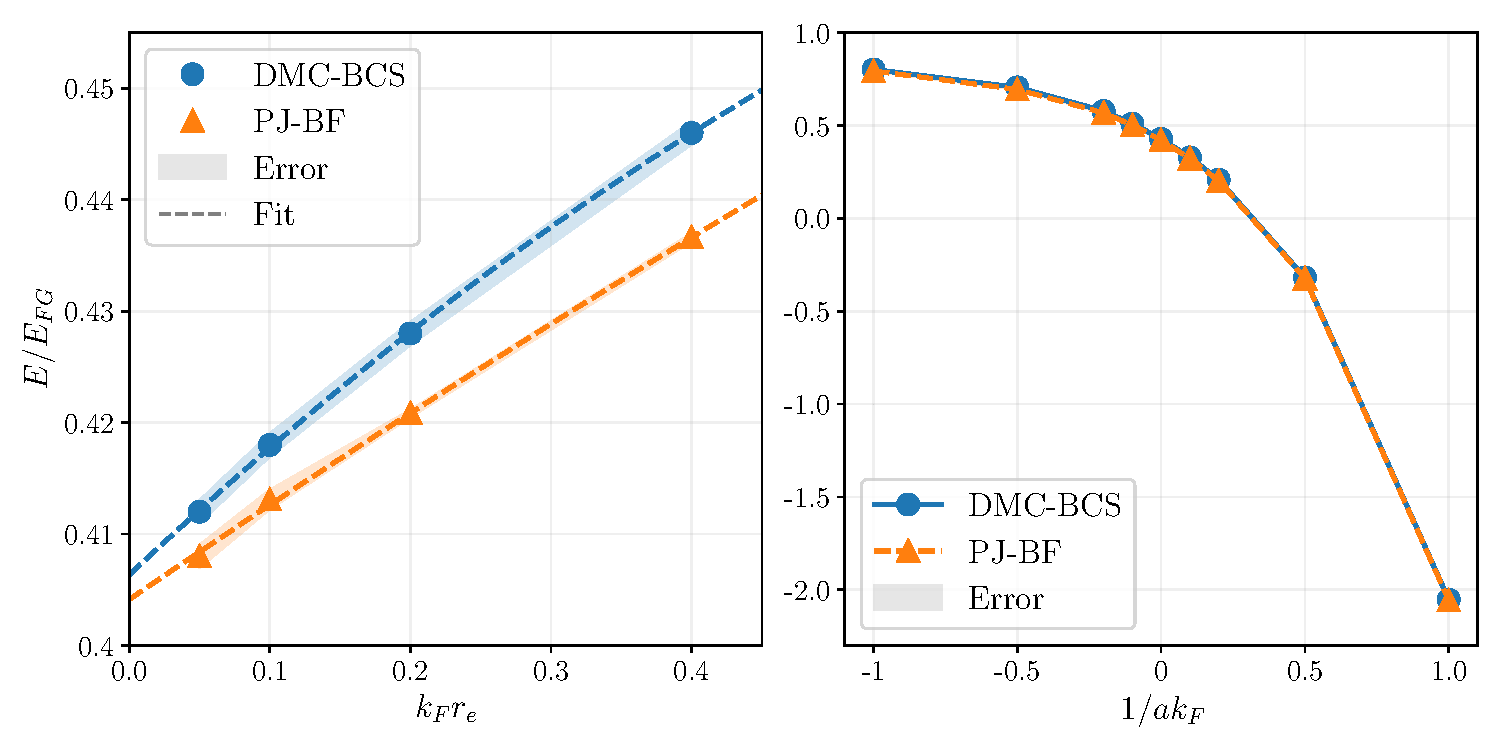
\includegraphics[width=0.75\columnwidth]{figures/condensed_matter/energies_reff_a.pdf}
\caption{Ground-state energy per particle of the UFG, normalized by the noninteracting Fermi gas energy in the thermodynamic limit, $E_{FG}$, as a function of effective range \(k_F r_e\) (left panel) and inverse scattering length \(1/(a k_F)\) (right panel).
Details of the calculations and uncertainty estimates are discussed in the main text.
}
\label{fig:ufg-energies-reff-a}
\end{figure}

\iffalse
As discussed in Sections~\ref{subsub:pfaffian_jastrow} and~\ref{sub:heg}, Ref.~\cite{kim_neural-network_2024} employs a Pfaffian--Jastrow NQS combined with a permutation-equivariant message-passing neural network. As shown in Figs.~\ref{fig:ufg-energies-T-N} and~\ref{fig:ufg-energies-reff-a}, the resulting variational energies are benchmarked against DMC calculations employing fixed-node constraints derived from BCS trial wave functions. Across the BCS--BEC crossover, for multiple particle numbers and in the extrapolation to zero effective range, the Pfaffian--Jastrow neural quantum state consistently yields lower energies than both Slater--Jastrow neural ans\"atze and state-of-the-art fixed-node DMC results.
\fi

As discussed in Sections~\ref{subsub:pfaffian_jastrow} and~\ref{sub:heg}, Ref.~\cite{kim_neural-network_2024} employs a Pfaffian--Jastrow NQS combined with a permutation-equivariant message-passing neural network. The ground-state energy per particle, normalized by the noninteracting Fermi gas energy in the thermodynamic limit, is shown in Figs.~\ref{fig:ufg-energies-T-N} and~\ref{fig:ufg-energies-reff-a}. For the NQS results, converged energies are obtained by averaging over the final 100 optimization iterations, with shaded bands indicating the corresponding standard deviations. DMC uncertainty bands correspond to standard errors extracted from block-averaged energies.

Figure~\ref{fig:ufg-energies-T-N} presents an initial comparison of three NQS architectures and two DMC benchmarks as a function of MPNN depth \(T\). The NQS architectures include Slater--Jastrow ans\"atze with plane-wave orbitals (SJ--PW) and with backflow correlations (SJ--BF), together with the Pfaffian--Jastrow (PJ--BF) ansatz. In the left panel, the interaction parameters are fixed such that \(k_F r_e = 0.4\), and DMC reference energies with (DMC--BCS) and without (DMC--PW) pairing are shown for comparison.
As the MPNN depth increases, the SJ--PW energies approach the DMC--PW benchmark, indicating that the MPNN captures correlations at a level comparable to DMC with a restricted nodal surface. 
However, incorporating backflow correlations generated by the MPNN into the single-particle orbitals of the Slater determinant, as in the SJ--BF ansatz, is still insufficient to capture the strong pairing correlations.
By contrast, the PJ--BF ansatz, which explicitly encodes these pairing correlations, outperforms DMC--BCS at all message-passing depths shown.
The right panel shows the system-size dependence of the energy at fixed effective range \(k_F r_e = 0.2\). Since all the MLPs used to construct the PJ--BF ansatz act only on pairs or single particles, the number of variational parameters does not explicitly depend on the particle number. For all particle numbers shown, the Pfaffian--Jastrow ansatz systematically yields lower energies than the DMC--BCS reference, with the difference between the two energies growing as the number of particles increases.



Figure~\ref{fig:ufg-energies-reff-a} shows energies at unitarity as a function of effective range, including extrapolations to zero effective range using quadratic fits, as well as results across the BCS--BEC crossover at fixed \(k_F r_e = 0.2\). These results demonstrate that the Pfaffian--Jastrow ansatz is robust across all parameter regions explored, indicating that the Pfaffian pairing structure provides a consistently more accurate variational description of strongly correlated pairing physics for ultracold Fermi gases near the unitary limit.


A central practical outcome of this work is the demonstration that transfer learning can stabilize and accelerate optimization in regimes characterized by strong, short-range interactions and small effective ranges. Because the ansatz does not encode explicit assumptions about short-distance structure, it remains broadly applicable. By progressively pretraining on softer interactions and smaller systems, a single unified ansatz can be extended to harder regimes and larger particle numbers, enabling a controlled exploration of the BCS--BEC crossover and finite-size effects.

Beyond ground-state energies, the Pfaffian--Jastrow NQS accurately describes observables sensitive to the quality of the variational wave function, including pair distribution functions and pairing gaps. The predicted pairing gaps are closer to experimental values than those obtained from DMC calculations based on BCS trial states, and are consistent within uncertainties with DMC results for substantially larger systems. This highlights the potential of neural-network-based Pfaffian ans\"atze for providing a faithful description of both energetic and pairing properties in strongly correlated fermionic systems.




